\chapter{Tables and Graphics}

\section{Tables}
	The following section contains examples of tables, most of which have been commented out for brevity. (They will show up in the .tex document in red, but not at all in the .pdf). For more help in constructing a table (or anything else in this document), please see the LaTeX pages on the CUS site. 

\begin{table}[htdp] % begins the table floating environment. This enables LaTeX to fit the table where it works best and lets you add a caption.
\caption[Basic Table 1]{A Basic Table: Correlation of Factors between Parents and Child, Showing Inheritance} 
% The words in square brackets of the caption command end up in the Table of Tables. The words in curly braces are the caption directly over the table.
\begin{center} 
% makes the table centered
\begin{tabular}{c c c c} 
% the tabular environment is used to make the table itself. The {c c c c} specify that the table will have four columns and they will all be center-aligned. You can make the cell contents left aligned by replacing the Cs with Ls or right aligned by using Rs instead. Add more letters for more columns, and pipes (the vertical line above the backslash) for vertical lines. Another useful type of column is the p{width} column, which forces text to wrap within whatever width you specify e.g. p{1in}. Text will wrap badly in narrow columns though, so beware.
\toprule % a horizontal line, slightly thicker than \hline, depends on the booktabs package
  Factors &  Correlation between Parents \& Child & Inherited \\ % the first row of the table. Separate columns with ampersands and end the line with two backslashes. An environment begun in one cell will not carry over to adjacent rows.
  \midrule % another horizontal line
Education & -0.49 & Yes \\ % another row
Socio-Economic Status & 0.28 & Slight \\
Income & 0.08 & No\\
Family Size & 0.19 & Slight \\
Occupational Prestige &0.21 & Slight \\
\bottomrule % yet another horizontal line
\end{tabular}
\end{center}
\label{inheritance} % labels are useful when you have more than one table or figure in your document. See our online documentation for more on this.
\end{table}

	\clearpage 
%% \clearpage ends the page, and also dumps out all floats. 
%% Floats are things like tables and figures.

If you want to make a table that is longer than a page, you will want to use the longtable environment. Uncomment the table below to see an example, or see our online documentation.

	\begin{longtable}{||c|c|c|c||}
	 	\caption[Long Table]{An example of a long table, with headers that repeat on each subsequent page: Results from the summers of 1998 and 1999 work at Reed College done
by Grace Brannigan, Robert Holiday and Lien Ngo in 1998 and Kate Brown and
Christina Inman in 1999.}\\ \hline
	    	  \multicolumn{4}{||c||}{Chromium Hexacarbonyl} \\\hline
		   State & Laser wavelength & Buffer gas & Ratio of $\frac{\textrm{Intensity
at vapor pressure}}{\textrm{Intensity at 240 Torr}}$ \\ \hline
		  \endfirsthead
		\hline     State & Laser wavelength & Buffer gas & Ratio of
$\frac{\textrm{Intensity at vapor pressure}}{\textrm{Intensity at 240 Torr}}$\\
\hline
		    \endhead

	    $z^{7}P^{\circ}_{4}$ & 266 nm & Argon & 1.5 \\\hline
	    $z^{7}P^{\circ}_{2}$ & 355 nm & Argon & 0.57 \\\hline
	    $y^{7}P^{\circ}_{3}$ & 266 nm & Argon & 1 \\\hline
	    $y^{7}P^{\circ}_{3}$ & 355 nm & Argon & 0.14 \\\hline
	    $y^{7}P^{\circ}_{2}$ & 355 nm & Argon & 0.14 \\\hline
	    $z^{5}P^{\circ}_{3}$ & 266 nm & Argon & 1.2 \\\hline
	    $z^{5}P^{\circ}_{3}$ & 355 nm & Argon & 0.04 \\\hline
	    $z^{5}P^{\circ}_{3}$ & 355 nm & Helium & 0.02 \\\hline
	    $z^{5}P^{\circ}_{2}$ & 355 nm & Argon & 0.07 \\\hline
	    $z^{5}P^{\circ}_{1}$ & 355 nm & Argon & 0.05 \\\hline
	    $y^{5}P^{\circ}_{3}$ & 355 nm & Argon & 0.05, 0.4 \\\hline
	    $y^{5}P^{\circ}_{3}$ & 355 nm & Helium & 0.25 \\\hline
	    $z^{5}F^{\circ}_{4}$ & 266 nm & Argon & 1.4 \\\hline
	    $z^{5}F^{\circ}_{4}$ & 355 nm & Argon & 0.29 \\\hline
	    $z^{5}F^{\circ}_{4}$ & 355 nm & Helium & 1.02 \\\hline
	    $z^{5}D^{\circ}_{4}$ & 355 nm & Argon & 0.3 \\\hline
	    $z^{5}D^{\circ}_{4}$ & 355 nm & Helium & 0.65 \\\hline
	    $y^{5}H^{\circ}_{7}$ & 266 nm & Argon & 0.17 \\\hline
	    $y^{5}H^{\circ}_{7}$ & 355 nm & Argon & 0.13 \\\hline
	    $y^{5}H^{\circ}_{7}$ & 355 nm & Helium & 0.11 \\\hline
	    $a^{5}D_{3}$ & 266 nm & Argon & 0.71 \\\hline
	    $a^{5}D_{2}$ & 266 nm & Argon & 0.77 \\\hline
	    $a^{5}D_{2}$ & 355 nm & Argon & 0.63 \\\hline
	    $a^{3}D_{3}$ & 355 nm & Argon & 0.05 \\\hline
	    $a^{5}S_{2}$ & 266 nm & Argon & 2 \\\hline
	    $a^{5}S_{2}$ & 355 nm & Argon & 1.5 \\\hline
	    $a^{5}G_{6}$ & 355 nm & Argon & 0.91 \\\hline
	    $a^{3}G_{4}$ & 355 nm & Argon & 0.08 \\\hline
	    $e^{7}D_{5}$ & 355 nm & Helium & 3.5 \\\hline
	    $e^{7}D_{3}$ & 355 nm & Helium & 3 \\\hline
	    $f^{7}D_{5}$ & 355 nm & Helium & 0.25 \\\hline
	    $f^{7}D_{5}$ & 355 nm & Argon & 0.25 \\\hline
	    $f^{7}D_{4}$ & 355 nm & Argon & 0.2 \\\hline
	    $f^{7}D_{4}$ & 355 nm & Helium & 0.3 \\\hline
	    \multicolumn{4}{||c||}{Propyl-ACT} \\\hline
%	    State & Laser wavelength & Buffer gas & Ratio of $\frac{\textrm{Intensity
%at vapor pressure}}{\textrm{Intensity at 240 Torr}}$\\ \hline
	    $z^{7}P^{\circ}_{4}$ & 355 nm & Argon & 1.5 \\\hline
	    $z^{7}P^{\circ}_{3}$ & 355 nm & Argon & 1.5 \\\hline
	    $z^{7}P^{\circ}_{2}$ & 355 nm & Argon & 1.25 \\\hline
	    $z^{7}F^{\circ}_{5}$ & 355 nm & Argon & 2.85 \\\hline
	    $y^{7}P^{\circ}_{4}$ & 355 nm & Argon & 0.07 \\\hline
	    $y^{7}P^{\circ}_{3}$ & 355 nm & Argon & 0.06 \\\hline
	    $z^{5}P^{\circ}_{3}$ & 355 nm & Argon & 0.12 \\\hline
	    $z^{5}P^{\circ}_{2}$ & 355 nm & Argon & 0.13 \\\hline
	    $z^{5}P^{\circ}_{1}$ & 355 nm & Argon & 0.14 \\\hline
	    \multicolumn{4}{||c||}{Methyl-ACT} \\\hline
%	    State & Laser wavelength & Buffer gas & Ratio of $\frac{\textrm{Intensity
% at vapor pressure}}{\textrm{Intensity at 240 Torr}}$\\ \hline
	    $z^{7}P^{\circ}_{4}$ & 355 nm & Argon & 1.6, 2.5 \\\hline
	    $z^{7}P^{\circ}_{4}$ & 355 nm & Helium & 3 \\\hline
	    $z^{7}P^{\circ}_{4}$ & 266 nm & Argon & 1.33 \\\hline
	    $z^{7}P^{\circ}_{3}$ & 355 nm & Argon & 1.5 \\\hline
	    $z^{7}P^{\circ}_{2}$ & 355 nm & Argon & 1.25, 1.3 \\\hline
	    $z^{7}F^{\circ}_{5}$ & 355 nm & Argon & 3 \\\hline
	    $y^{7}P^{\circ}_{4}$ & 355 nm & Argon & 0.07, 0.08 \\\hline
	    $y^{7}P^{\circ}_{4}$ & 355 nm & Helium & 0.2 \\\hline
	    $y^{7}P^{\circ}_{3}$ & 266 nm & Argon & 1.22 \\\hline
	    $y^{7}P^{\circ}_{3}$ & 355 nm & Argon & 0.08 \\\hline
	    $y^{7}P^{\circ}_{2}$ & 355 nm & Argon & 0.1 \\\hline
	    $z^{5}P^{\circ}_{3}$ & 266 nm & Argon & 0.67 \\\hline
	    $z^{5}P^{\circ}_{3}$ & 355 nm & Argon & 0.08, 0.17 \\\hline
	    $z^{5}P^{\circ}_{3}$ & 355 nm & Helium & 0.12 \\\hline
	    $z^{5}P^{\circ}_{2}$ & 355 nm & Argon & 0.13 \\\hline
	    $z^{5}P^{\circ}_{1}$ & 355 nm & Argon & 0.09 \\\hline
	    $y^{5}H^{\circ}_{7}$ & 355 nm & Argon & 0.06, 0.05 \\\hline
	    $a^{5}D_{3}$ & 266 nm & Argon & 2.5 \\\hline
	    $a^{5}D_{2}$ & 266 nm & Argon & 1.9 \\\hline
	    $a^{5}D_{2}$ & 355 nm & Argon & 1.17 \\\hline
	    $a^{5}S_{2}$ & 266 nm & Argon & 2.3 \\\hline
	    $a^{5}S_{2}$ & 355 nm & Argon & 1.11 \\\hline
	    $a^{5}G_{6}$ & 355 nm & Argon & 1.6 \\\hline
	    $e^{7}D_{5}$ & 355 nm & Argon & 1 \\\hline

		\end{longtable}

   
   \section{Figures}
   
	If your thesis has a lot of figures, \LaTeX\ might behave better for you than that other word processor.  One thing that may be annoying is the way it handles ``floats'' like tables and figures. \LaTeX\ will try to find the best place to put your object based on the text around it and until you're really, truly done writing you should just leave it where it lies.   There are some optional arguments to the figure and table environments to specify where you want it to appear; see the comments in the first figure.

	If you need a graphic or tabular material to be part of the text, you can just put it inline. If you need it to appear in the list of figures or tables, it should be placed in the floating environment. 
	
	To get a figure from StatView, JMP, SPSS or other statistics program into a figure, you can print to pdf or save the image as a jpg or png. Precisely how you will do this depends on the program: you may need to copy-paste figures into Photoshop or other graphic program, then save in the appropriate format.
	
	Below we have put a few examples of figures. For more help using graphics and the float environment, see our online documentation.
	
	And this is how you add a figure with a graphic:
	\begin{figure}[h]
	% the options are h = here, t = top, b = bottom, p = page of figures.
	% you can add an exclamation mark to make it try harder, and multiple
	% options if you have an order of preference, e.g.
	% \begin{figure}[h!tbp]
	   
	       \centering
	    % DO NOT ADD A FILENAME EXTENSION TO THE GRAPHIC FILE
	    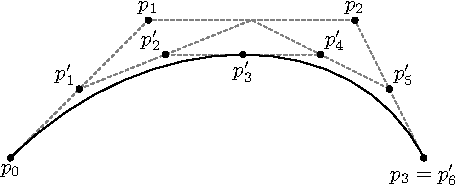
\includegraphics{subdivision}
	     \caption{A Figure}
	 \label{subd}
	\end{figure}

\clearpage %% starts a new page and stops trying to place floats such as tables and figures

\section{More Figure Stuff}
You can also scale and rotate figures.
 	\begin{figure}[h!]
	   
	       \centering
	    % DO NOT ADD A FILENAME EXTENSION TO THE GRAPHIC FILE
	    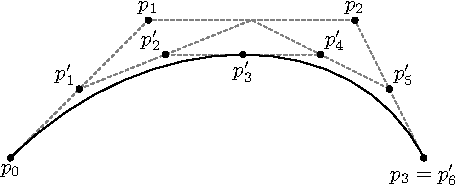
\includegraphics[scale=0.5,angle=180]{subdivision}
	    % if your figure shows up not where you want it, it may just be too big to fit. You can use the scale argument to shrink it, e.g. scale=0.85 is 85 percent of the original size. 
	     \caption{A Smaller Figure, Flipped Upside Down}
	 \label{subd2}
	\end{figure}

\section{Even More Figure Stuff}
With some clever work you can crop a figure, which is handy if (for instance) your EPS or PDF is a little graphic on a whole sheet of paper. The viewport arguments are the lower-left and upper-right coordinates for the area you want to crop.

 	\begin{figure}[h!]
	    	       \centering
	    % DO NOT ADD A FILENAME EXTENSION TO THE GRAPHIC FILE
	   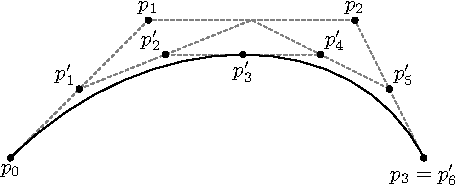
\includegraphics[clip=true, viewport=.0in .0in 1in 1in]{subdivision}
	    \caption{A Cropped Figure}
	 \label{subd3}
	\end{figure}
	
      \subsection{Common Modifications}
      The following figure features the more popular changes thesis students want to their figures. This information is also on the web at \url{web.reed.edu/cis/help/latex/graphics.html}.
           \renewcommand{\thefigure}{0.\arabic{figure}} %Renumbers the figure to the type 0.x
    \addtocounter{figure}{4} %starts the figure numbering at 4
    \begin{figure}[htbp]
    \begin{center}
   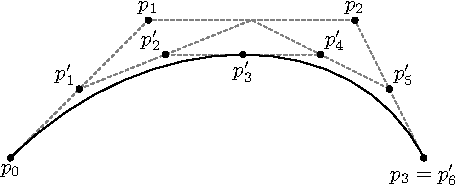
\includegraphics[scale=0.5]{subdivision}
    \caption[Flower type and percent specialization]{\footnotesize{Interaction bar plot showing the degree of specialization for each flower type.}} %the special ToC caption is in square brackets. The \footnotesize makes the figure caption smaller
    \label{barplot}
    \end{center}
    \end{figure} 